\setchapterpreamble[u]{\margintoc}
\chapter{Findings: Mobile Analytics Tools and their Artefacts}~\label{chapter-tools-and-their-artefacts}
This chapter covers two of the six perspectives, \emph{i.e.} using and improving mobile analytics tools. The primary evidence comes from both the app-centric and the tool-centric case studies, augmented with material from grey data and grey literature.

The evidence has been analysed and prioritised to keep the chapter relatively succinct and on topic. 38 discrete themes (L1 themes) emerged in the analysis of the evidence, of these the 18 with strongest support in terms of the evidence are included here, the rest would benefit from further work. The L1 themes included in this chapter have be aggregated into four higher-level (L2) themes: design (\secref{section-design}), fit-for-purpose (\secref{section-fit-for-purpose}), utility (\secref{section-utility}), dependability (\secref{section-dependability}). Figure \ref{fig:analytics-tools-and-their-artefacts-fishbone-diagram} illustrates the top L1 themes and their primary higher-level (L2) theme.

\begin{figure}
    \centering
    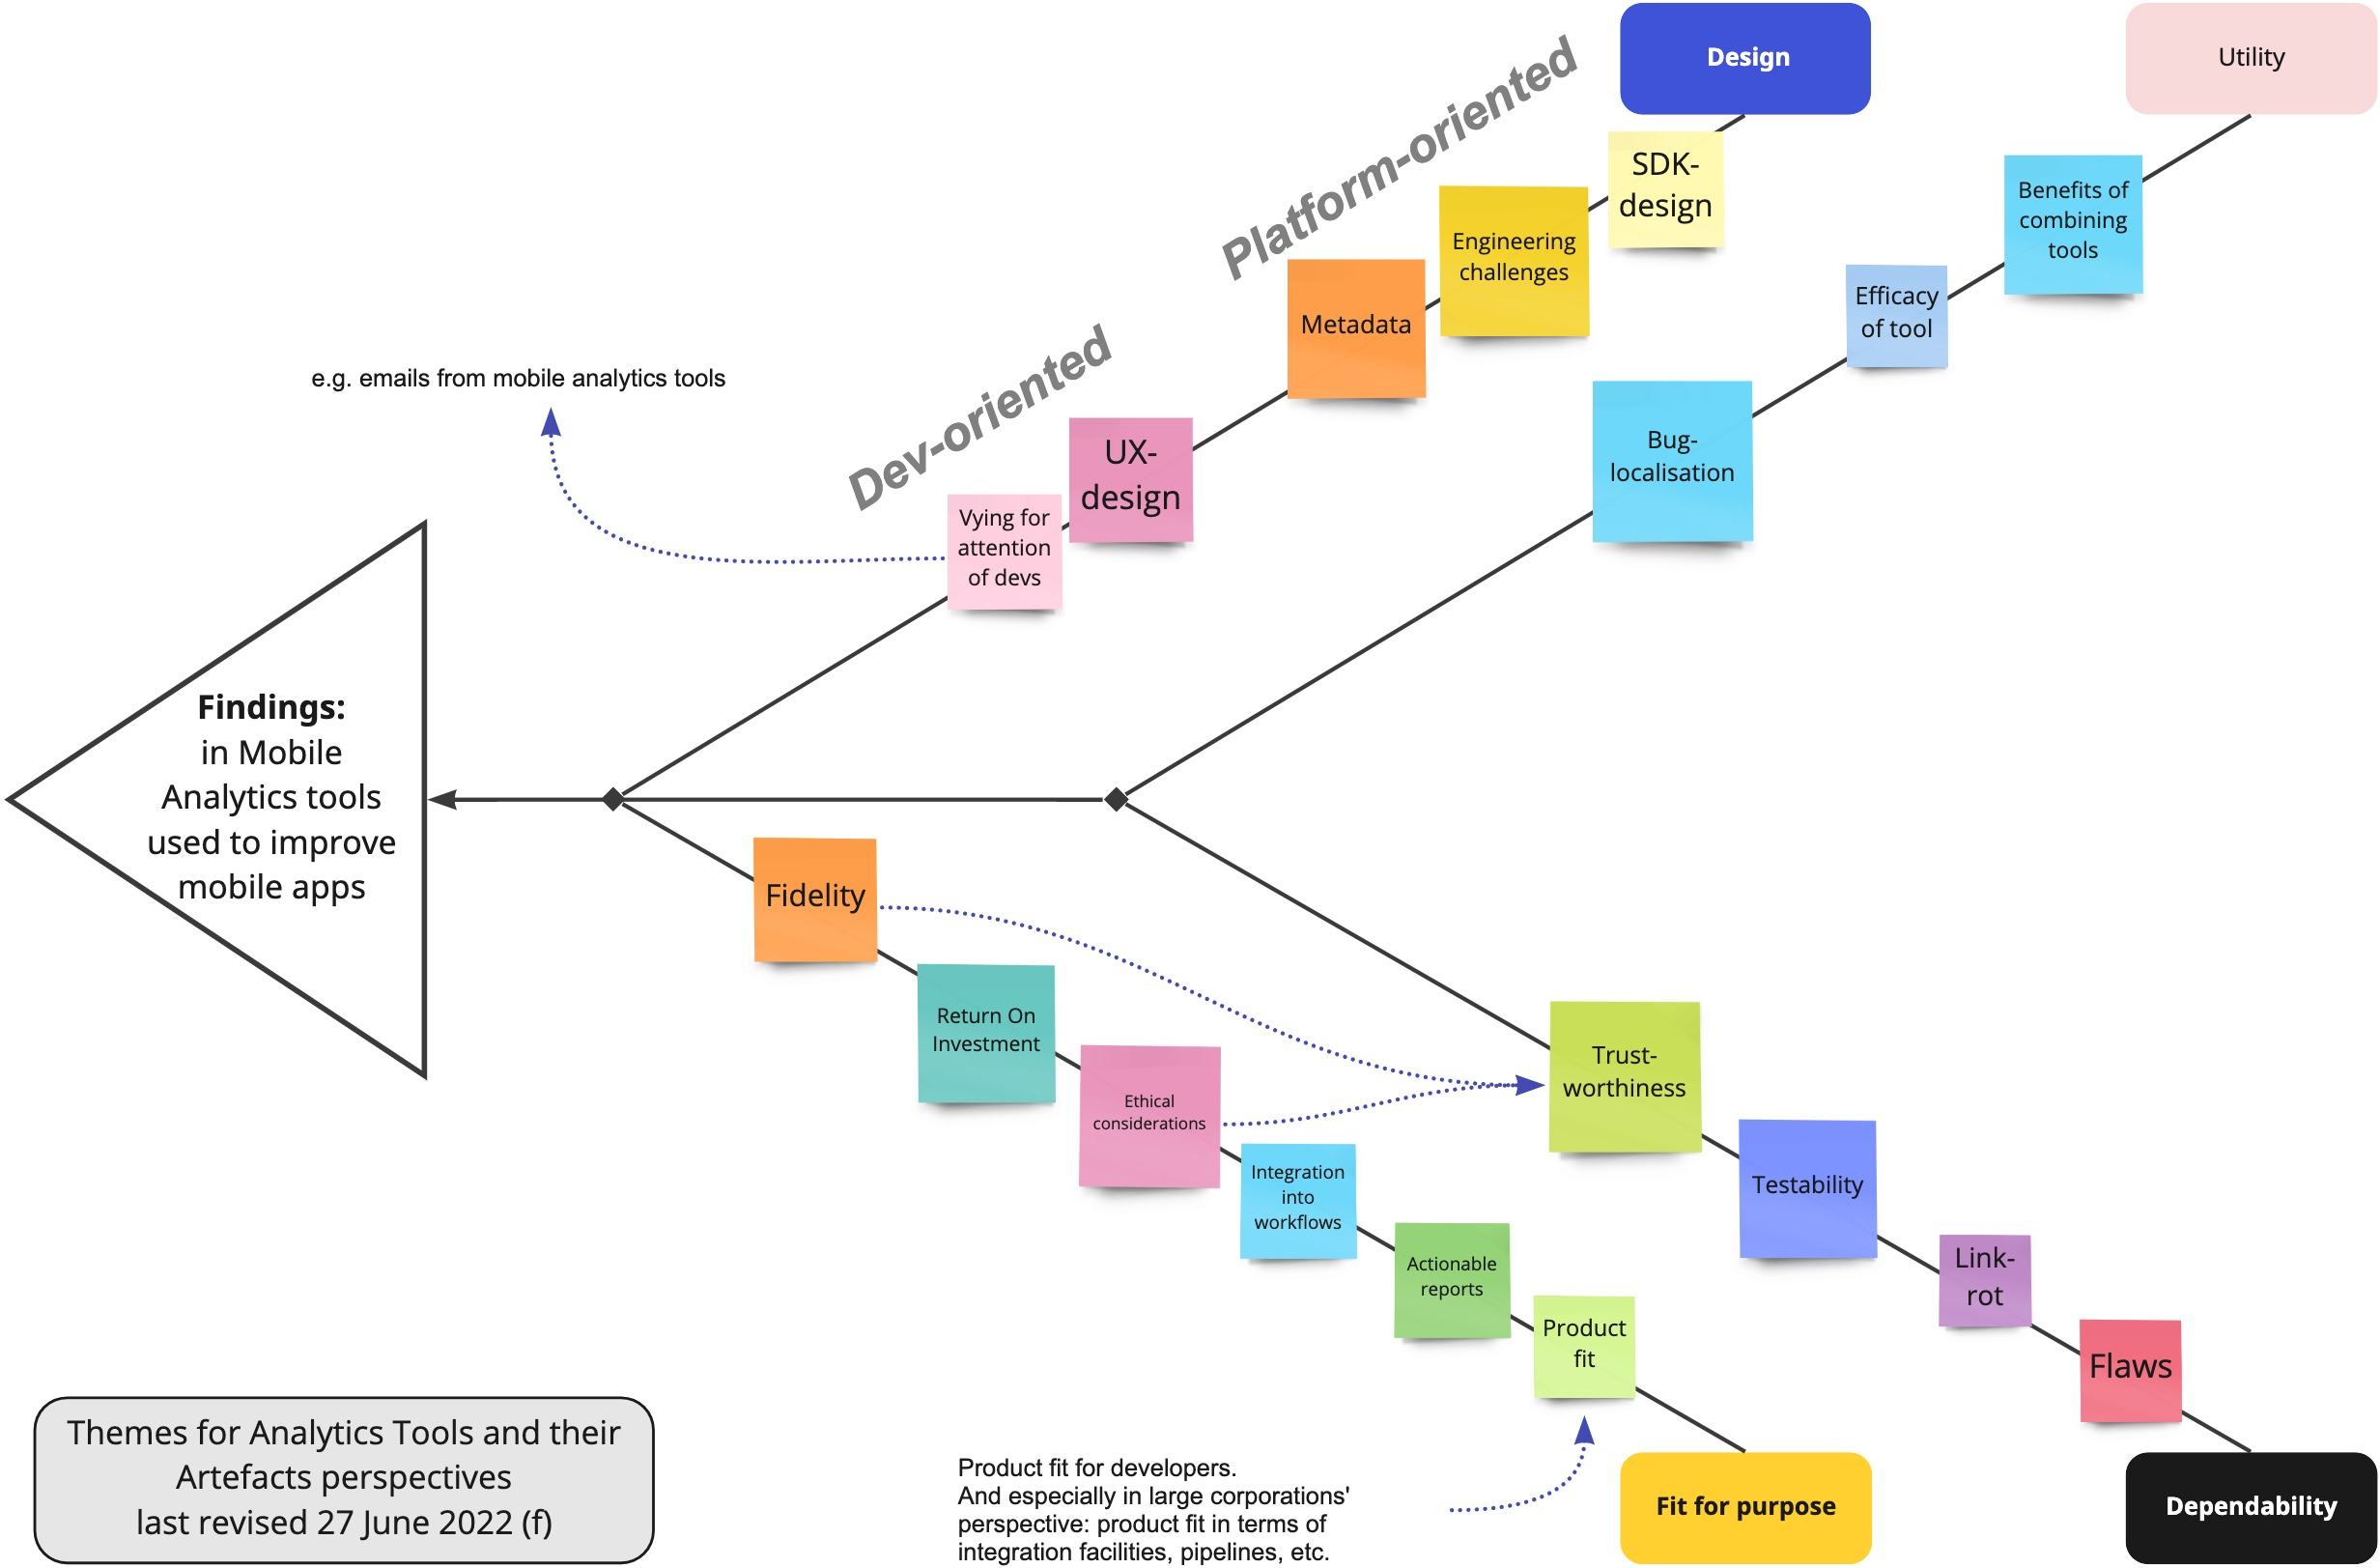
\includegraphics[width=\textwidth]{images/rough-sketches/analytics-tools-and-their-artefacts-fishbone-diagram-27-jun-2022f.jpeg}
    \caption{Analytics Tools and their Artefacts Fishbone Diagram\\Source: \href{https://miro.com/app/board/uXjVOtIsyWo=/?share_link_id=293061080490}{Miro}}
    \label{fig:analytics-tools-and-their-artefacts-fishbone-diagram}
\end{figure}

\section{Design}~\label{section-design}~\label{tata-chapter-section-design}
Design emerged as by far the most pertinent topic for the mobile analytics tools. There are two key, connected facets: 


\begin{itemize}
\item the design of the on-device \Gls{sdk}, including addressing various engineering challenges and deciding on the meta-data to collect; and 
\item UX design to engage the developers to actually use the results of the mobile analytics [effectively].
\end{itemize}

The design of the on-device SDK is important because any in-app SDK needs to integrate easily in to the mobile app, and platform-level analytics need to be seamless and collect sufficient pertinent information to be useful for the app developers. They also need to be robust and timely in terms of collection, transmission, and processing of the underlying data in order for developers to have timely access to the results.

Mobile Analytics tools need to be used to be effective, and the user experience of the developers who use these tools where \emph{``developers’ needs are characterized by efficiency, informativeness, intuitiveness, and flexibility of the tool.''}~\sidecite[][p. 104]{kuusinen2016_flow_intrinsic_motivation_and_developer_experience_in_sw_eng}. Where using a tool is rewarding for the developers they are likely to use the tool more~\sidecite[][p. 260]{kuusinen2016_are_sw_devs_just_users_of_devt_tools_etc}.

These tools are a subset of software trying to get a developer's attention and they need to fit within a larger context. The tools need to surface (make visible) functionality and capabilities that align with the motivation(s) of the developers~\sidecite[][p. 2]{zaina2021_ux_information_in_the_daily_work_of_an_agile_team}.

\myindex{Fabric Crashlytics} is an archetypal example of how a mobile analytics tool can be designed to serve developers well. The product team developed it from the ground up, starting with excellent crash reporting, to provide developers with timely, actionable, attractive, and useful reports. This led to it becoming one of the top three mobile analytics tools for both iOS and Android within 10 months of being launched~\sidecite{___answersblog_2015_may_crashlytics-no1-in-performance}. % See also https://web.archive.org/web/20151203150947/http://fabric.io/blog/crashlytics-answers-named-top-mobile-sdks
First Twitter acquired it and then Google did; they subsequently integrated it into \myindex{Firebase Analytics} which is the most popular mobile analytics service for Android apps currently. 

It exemplified good design in terms of the SDK as it collected pertinent data developers found useful without requiring significant effort by the developers. The development team who created the SDK and the product had used their frustrations from using other analytics software as a catalyst to create Crashlytics. 

Similarly the user-interface of Crashlytics was slick from the outset and quickly adopted by app developers through presenting the analysis of the data the SDK had collected. It was designed from the outset to be actionable save \emph{`developers from information overload or ``analysis paralysis'''}~\sidecite{burke2014_wayne_chang_interview}.

Developers found it useful, it was free of charge, and the product continued to evolve and improve rapidly, for example by adding a general purpose mobile analytics service, called Answers, to Crashlytics that, in their words: \emph{``Before Answers, developers had to wade through mountains of data about their apps to find what they were looking for. We wanted to fix this, so we went to the drawing board and set out to build a mobile analytics solution you didn’t need to analyze.''}~\sidecite{___answersblog_2015_may_crashlytics-no1-in-performance} 

\section{\itools}


\section{Fieldstones}
\julian{These need integrating or removing pre-submission.}

An interesting phenomenon observed during the Catrobat hackathon where some of the crashes that appeared in Android Vitals were believed to come from `soft errors' in the Pocket Code app. The issue, CATROID-426, was logged during the hackathon~\sidecite{catroid_426_soft_crashes_should_not_be_reported_to_the_play_console} and the developers wrote two sets of code changes (also known as `commits'). These were merged into the app's codebase on \nth{21} Nov 2019 and released in the Pocket Code app several weeks later.

The intent was laudable, however, at least some of the soft crashes continued to occur over a month later, as documented in \url{https://jira.catrob.at/browse/CATROID-422}. This issue was raised in the hackathon and closed as a duplicate by one of the developers involved in trying to stop the soft errors from appearing in Android Vitals \sidecite{catroid_426_soft_crashes_should_not_be_reported_to_the_play_console}.

TODO Mention the Pocket Code experience when migrating from Fabric to Firebase and the additional, unexpected analytics that appeared. Forward reference to the discussion on intrusiveness.

\itools \myindex{iTools} simple facilities such as the ability to search through the failures to find any failure clusters that match. A recent example is searching for instances of an \texttt{IndexOutOfBoundsException} in the \myindex{Kiwix} custom apps\sidenote{\href{https://github.com/kiwix/kiwix-android/issues/2542}{Index Out of Bounds Exception on Custom App \#2542}} where \myindex{Android Vitals} had to be checked page by page for each app to see if the crash was still happening.

Aggregation and mining across the matching clusters would also be useful. Tagging/labelling might also help, \emph{ditto} facilities to cross-reference within and across systems (\emph{c.f.} hyperlinking and reference links.

A placeholder until the relevant content is added to check the formatting in the index for: Android Vitals\index{GitHub Projects!Android Vitals}

Breadcrumbs: in AppPulse Mobile iOS which provided similar capabilities in Android~\sidecite{microfocus2018_apppulse_mobile_android_getting_started_video, hp_apppulse_mobile_android_guide_v1_9} and iOS~\sidecite{freeman2016_apppulse_ios_mobile_example}.